\chapter{Voorgestelde testmethodiek }	\label{sec:methodiekvantesten}
Dit hoofdstuk behandelt de wijze waarop de testen naar consistentie en beschikbaarheid worden uitgevoerd. 
De methodiek is opgedeeld in 4 stappen: het opstellen, het kalibreren, het testen van de systemen en tenslotte het verzamelen en analyseren van de resultaten. Een overzicht van de procedure wordt weergegeven in figuur \ref{fig:test-process-overview}.

\paragraph{Opstellen van de testomgeving} De eerste stap bestaat uit het selecteren, installeren en configureren van een DBMS en de testsoftware. Een variatie in hardware van de systemen, versienummer van de software of een verschillende netwerkinfrastructuur kan de uiteindelijke testresultaten beïnvloeden. 

\paragraph{Kalibratie van de testomgeving} In de uiteindelijke testen wordt het gedrag onder matige belasting getest. Afhankelijk van de gekozen systemen en de netwerkinfrastructuur zal dit voor elke DBMS een verschillende hoeveelheid bewerkingen geven. Deze stap bepaalt welke queries er uitgevoerd worden, hoeveel gebruikers er zijn in het systeem en hoeveel bewerkingen er uitgevoerd worden per seconde. 

\paragraph{Testen van de systemen} In deze stap worden de testen op de verschillende systemen uitgevoerd. Deze methodiek maakt het mogelijk om te testen hoe de vertraging op een bewerking zich gedraagt voor, tijdens en na het falen en herstellen van een systeem. Voor de consistentie is het mogelijk om zowel een passieve als actieve analyse te doen. 

\paragraph{Verzamelen en analyseren van de testdata} In de laatste stap wordt de data van de vorige stappen verzameld en de resultaten visueel voorgesteld. Met behulp van de testdata, is het mogelijk om bepaalde conclusies te maken over de beschikbaarheids- en consistentiegaranties van de verschillende DBMS's. 

In de volgende secties worden de verschillende stappen uitgewerkt.  
\begin{figure}[ht!]
\centering
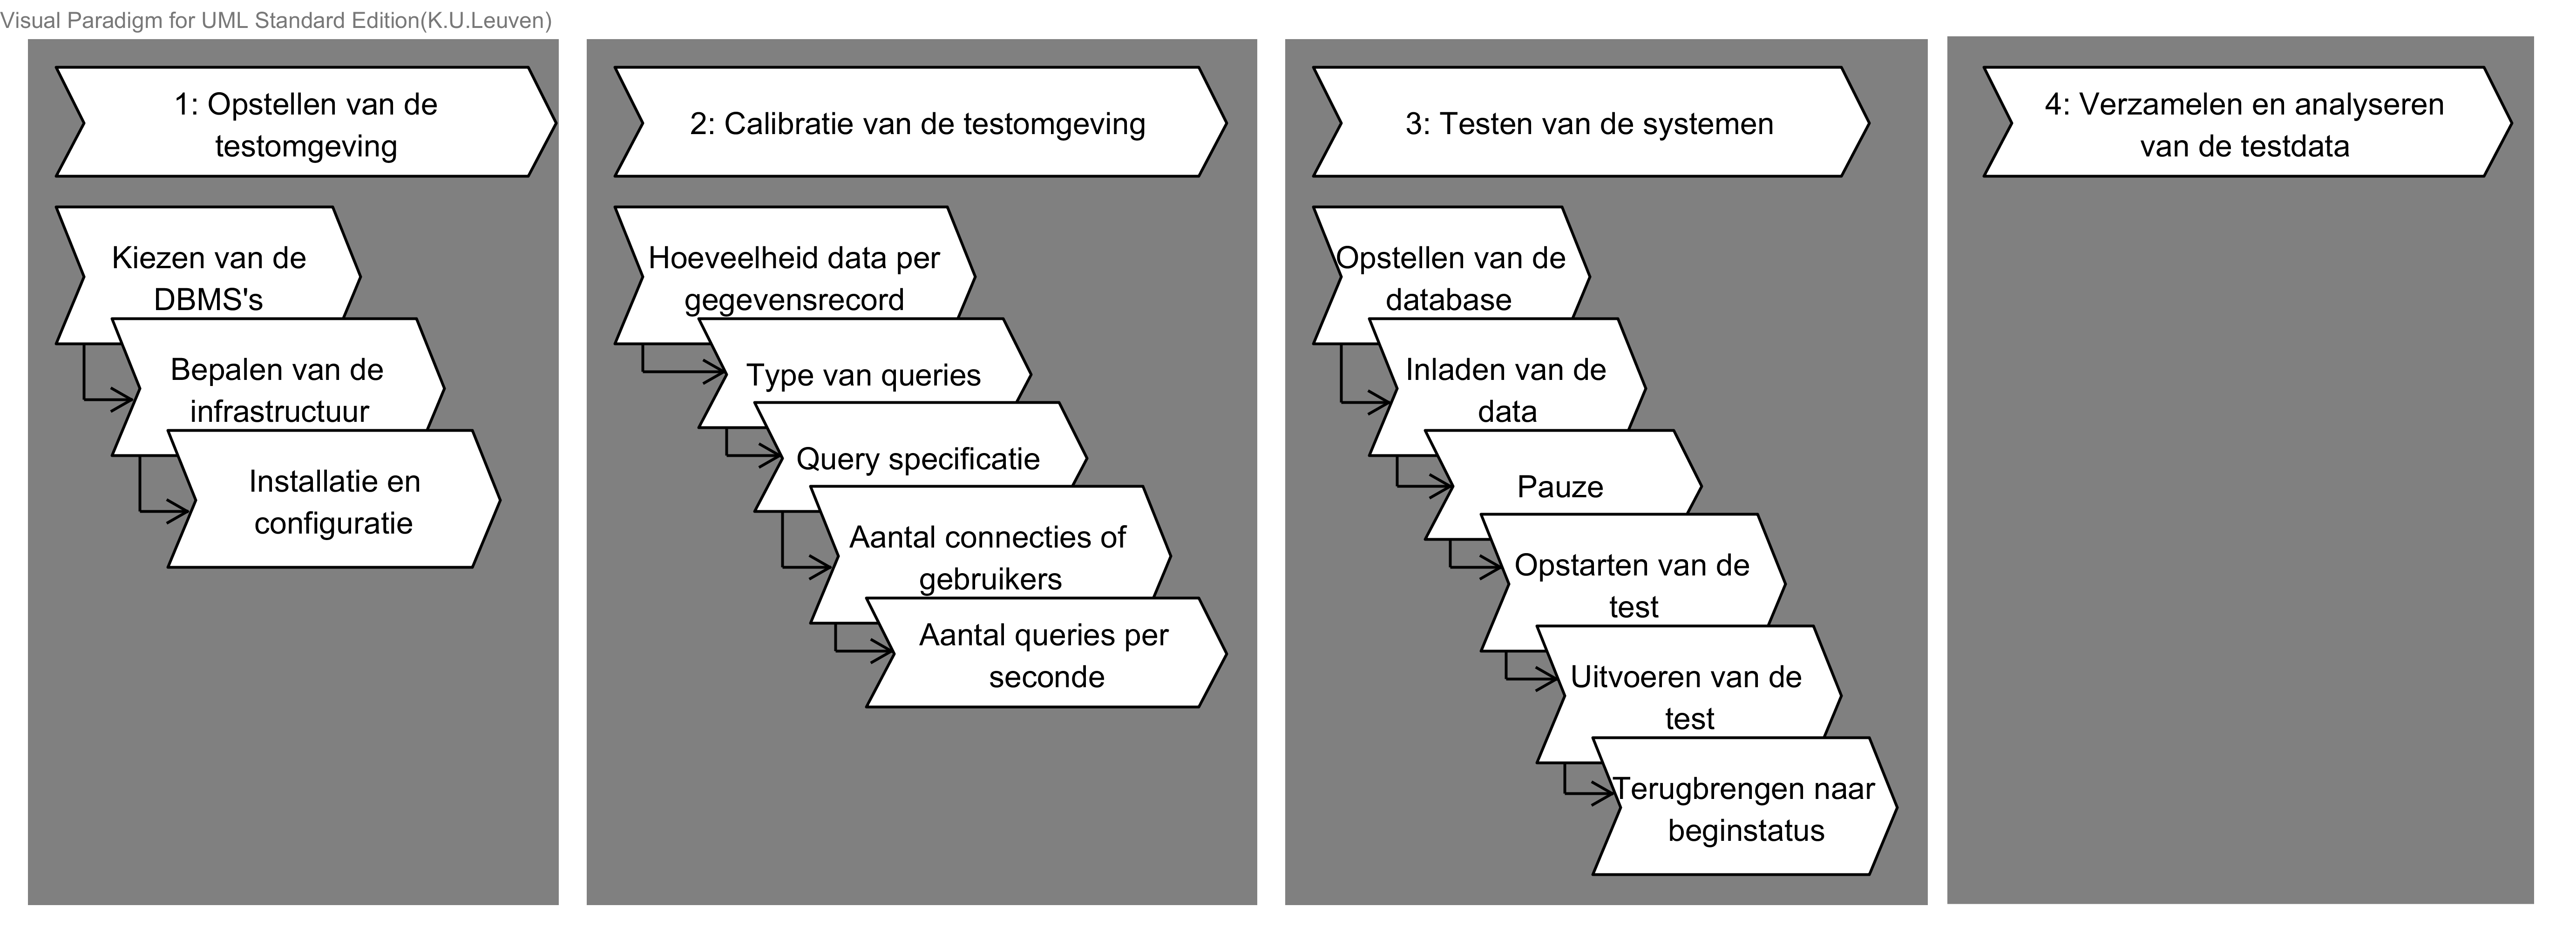
\includegraphics[width=\linewidth]{img/Test-Process-Detailed-Overview}
\caption{Een gedetailleerd overzicht van het testproces met al de verschillende stappen}
\label{fig:test-process-overview}
\end{figure}

\section{Stap 1: Opstellen van de testomgeving}
\paragraph{Keuze van DBMS's} In eerste instantie moet er gekozen worden welke DBMS's er getest worden. Er zijn verschillende mogelijke keuzes, er kan een enkele systeem getest worden in één configuraties of verschillende configuraties, er kunnen ook verscheidene database systemen naast elkaar besproken worden. 

\paragraph{Bepalen van de infrastructuur} Vervolgens gebeurt de keuze van de infrastructuur. Dit gebeurt door het aantal instanties per systeem vast te leggen en de hardware te kiezen. 

\paragraph{Installatie en configuratie} Het lokaal installeren en configureren van een softwarepakket is in Unix veelvuldig geautomatiseerd met behulp van tools zoals \textit{apt-get} en \textit{yum}. Voor een systeem in een gedistribueerde omgeving is de situatie ingewikkelder. In een gedistribueerd systeem, dienen de verschillende servers van elkaar op de hoogte gebracht.

Deze gedistribueerde configuratie stap staat in voor het in contact brengen van de verschillende services op de verschillende servers. Voor verschillende servics zijn er andere configuratie methodes, bij sommigen gebeurt dit door middel van configuratiebestanden voor het opstarten van de service. Bij andere gebeurt dit via de API na het opstarten van de services. 

Na het uitvoeren van deze stap, zou het DBMS moeten werken zoals vereist. 

\section{Stap 2: Kalibratie van de testomgeving}
Verschillende DBMS's ondersteunen een andere belasting aan, ook bij een zelfde DBMS zijn er grote verschillen bij het veranderen van de configuratie of de infrastructuur. Het de bedoeling dat alle database systeem een matige belasting te hebben bij de testen, op deze manier kan er gefocust worden op de consistentie en beschikbaarheid. Bij een hoge belasting wordt er meer gefocust op de performantie en is er een hogere vertraging. De queueing theorie geeft de eigenschap dat de totale vertraging (R) gelijk is aan de som van verwerkings- (S) en wachttijd (W)\cite{millsap2003optimizing}. Dit verband is visueel voorgesteld ten opzichte van de belasting in figuur \ref{fig:hockey-stick}. 

\begin{figure}[ht!] 
\centering
	\subfigure[Verband vertraging ten opzicht van de belasting van een DBMS.]{\label{fig:hockey-stick} 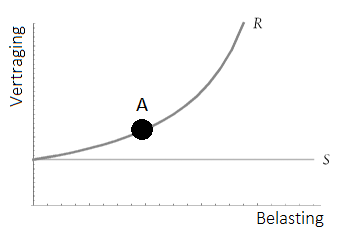
\includegraphics[width=0.45\textwidth]{img/hockey-stick}}
	\hfill
	\subfigure[Verband aantal requests/seconde ten opzicht van het aantal gebruikers.]{\label{fig:connecties-gebruikers} 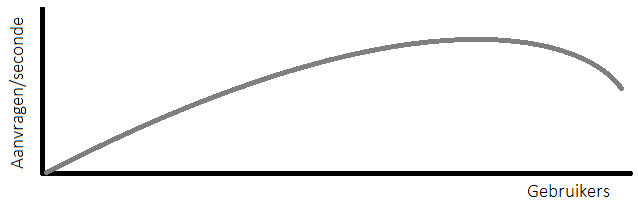
\includegraphics[width=0.45\textwidth]{img/connecties-gebruikers}}
	\caption{Verbanden voor de kalibratie}
\end{figure}
De belasting van een database is afhankelijk van verschillende parameters. In dit gedeelte wordt er gefocust op 5 groepen die in de benchmark tool geconfigureerd worden:

\paragraph{Hoeveelheid data per gegevensrecord} Elke record in de database kan bestaan uit verschillende kolommen met per kolom een waarde. Het is vereist om te definiëren hoe groot een gemiddeld kolom is en het aantal kolommen. Een klein record zorgt voor minder netwerkverkeer en een ander schijfgebruik dan een groot record. 

\paragraph{Type van queries} De opgeslagen data kan opgevraagd worden op verschillende wijze. Data kan ingevoegd, aangepast, opgevraagd of verwijderd worden. Daarbij kan dit telkens gebeuren voor 1 of meerdere records tegelijk. Afhankelijk van de relatieve verhouding, is er een andere belasting en vertraging: sommige DBMS's zijn meer geschikt voor een dominantie in leesacties, andere prefereren een dominantie in schrijfacties. Enkele systemen lezen data efficiënt in grote aantallen, andere lezen goed in kleine aantallen. 

\paragraph{Query specificatie} Bij het opvragen of verwijderen van een record, kan er een verschil zijn naar processing tijd afhankelijk hoe lang geleden de record geschreven of gelezen is en of naburige data onlangs gelezen is. Dit kan het geval zijn door caching methodes die het lezen van bepaalde records versnellen. Vandaar dat de distributie waarmee verschillende record gelezen en geschreven gekozen dient te worden. Voorbeelden van verschillende technieken zijn: voornamelijk de laatste data lezen, een uniforme kans voor alle data of bepaalde records regelmatig lezen.

\paragraph{Aantal connecties of gebruikers} Bij een gedistribueerde database systeem kunnen er meerdere gebruikers tegelijk actief zijn. Maar sommige systemen hebben een voorkeur naar weinig connecties met grote hoeveelheden data, andere kunnen meer gebruikers tegelijk behandelen. Het totaal aantal queries kan berekend worden als: $\#Queries = \#Gebruikers * \#QueriesPerGebruiker$. Bij het uitvoeren van deze test wordt er verondersteld dat elke gebruiker het maximaal aantal queries doet, dus $1/Vertraging$. Rekening houdend met de exponentiële groei van de wachtrij vertraging (figuur \ref{fig:hockey-stick}), betekent dit dat er een maximum aantal queries per seconde bereikt wordt bij een bepaald aantal gebruikers. In deze stap wordt er gezocht naar dit aantal gebruikers. De grafiek van het aantal gebruikers versus het aantal bewerkingen per second zal een gelijkaardig verloop hebben als de grafiek in figuur \ref{fig:connecties-gebruikers}. 

\paragraph{Aantal queries per seconde} In de vorige stap is er het optimale aantal gebruikers bepaald om het maximaal aantal bewerkingen uit te voeren. In het begin is er gesteld dat er gezocht wordt naar een matige belasting. Deze matige belasting komt overeen met punt A uit figuur \ref{fig:hockey-stick}. Op dit moment is er nog een lineaire verhouding tussen de wachttijd en de belasting. 

Met de parameters afkomstig uit de kalibratie, kunnen de testen opgestart en uitgevoerd worden. 

\section{Stap 3: Testen van de systemen} \label{sec:testenvandesystemen}
In deze thesis zullen er 2 verschillende soort testen uitgevoerd worden namelijk de beschikbaarheid en consistentietesten, welke dezelfde stappen volgen, elk met hun eigen specifieke parameters. Er zijn de 6 deelstappen: 

\paragraph{Opstellen van de database} In stap 2 was er gekozen voor een structuur van de data. Deze structuur wordt zo goed mogelijk meegegeven aan het DBMS zodat deze aan optimale schijfallocatie kan doen en de bewerkingen ook kan optimaliseren. Indien mogelijk dient ook meegegeven worden hoe de data opgevraagd zal worden, meestal gebeurt dit door middel van een bepaald veld die als sleutel zal gebruikt worden. 

\paragraph{Inladen van de data} Een bepaalde hoeveel data wordt vooraf ingeladen. Dit wordt gedaan om een basishoeveelheid data te hebben die nodig is voor de verdere initialisatie van de database. Verschillende DBMS's verdelen van de data over verschillende servers, dit wordt sharding genoemd. In bepaalde DBMS's gebeurt deze sharding pas bij het overschrijven van een bepaalde hoeveelheid records, om deze reden wordt er data ingeladen zodat deze sharding al is toegepast voor het opstarten van de eigenlijke testen. Dit inladen van de data gebeurt op maximale snelheid. 

\paragraph{Pauze} Na het inladen van de data wordt enige tijd gewacht. Zoals aangetoond in YCSB++\cite[Figuur 9]{patil2011ycsb++}, is er hogere vertraging in de DBMS's onmiddellijk na het schrijven van de data. Dit kan onder andere te wijten zijn doordat data nog weggeschreven moet worden naar schijf, gerepliceerd over verschillende servers of in bepaalde systemen zou het kunnen dat de sharding gebeurt op momenten met weinig belasting. Met het toevoegen van de wachtperiode wordt deze verhoogde belasting van de eigenlijke test weggehouden. 

\paragraph{Opstarten van de test (opstart kost)} De test wordt opgestart. In veel gevallen is er in het begin een opwarmfase nodig omdat de vertraging net hoger of lager is dan het gemiddelde. Deze hogere tijd is onder andere te verklaren door de connecties die opgezet moet worden en caches voor gelezen data die worden gevuld. Soms is deze lager omdat de schijf nog niet belast is of omdat er nog veel schrijfbuffers leeg zijn. Om dit gedrag te vermijden, wordt de data, verzameld in de eerste seconden, niet gebruikt voor de analyse. 

\paragraph{Uitvoeren van de test} De eigenlijke test wordt uitgevoerd, de data wordt verzameld en opgeslagen. De details van de beide testen volgen achteraf. 

\paragraph{Terugbrengen naar beginstatus} Na het uitvoeren van de test, wordt het DBMS terug naar de beginstatus gebracht. Onder andere de data en de database worden volledig verwijderd. Belangrijk in dit geval is het controleren of de data volledig verwijderd is, in bepaalde gevallen wordt de data enkel onzichtbaar gemaakt bij het verwijderen, hetgeen kan een volgende test kan beïnvloeden. 

De twee verschillende testmethodes zullen nu in detail behandeld worden. 
\subsection{Beschikbaarheidstest}
Bij de beschikbaarheidstest wordt er gekeken hoe het systeem reageert op tijdelijke, (on)verwachte onbeschikbaarheid van een deel van het systeem. In deze testen worden er 3 mogelijke oorzaken getest die de systemen onbeschikbaar maken, terwijl de belasting uit de kalibratiestap wordt toegepast. 

\paragraph{Zachte stop} De DMBS service wordt gevraagd om te stoppen. Op deze manier krijgt de service een signaal dat deze moet stoppen waarmee deze de andere kan waarschuwen, vervolgens zal de service stoppen. Achteraf wordt dezelfde service terug opgestart. Dit simuleert het gepland uitschakelen van een systeem. 

\paragraph{Harde stop} De DMBS service wordt onmiddellijk gestopt door het proces te beëindigen. De service heeft geen tijd om de andere te waarschuwen. Achteraf wordt dezelfde service terug opgestart. Dit simuleert een crash van de service die de systeembeheerders pas later opmerken en hij de service opnieuw opstart. 

\paragraph{Netwerk onderbreken} Al het in- en uitgaand netwerkverkeer wordt gestopt zonder enige waarschuwing. De service heeft geen tijd om de andere te waarschuwen én de zender krijgt geen onbereikbaar antwoord. Achteraf wordt het netwerk verkeer terug toegelaten. Dit simuleert een onderbroken internetverbinding of een gecrashte server.  

Eenzelfde DBMS kan sterk verschillend reageren op de verschillende situaties: de eerste situatie is het eenvoudigst te behandelen aangezien het systeem de andere op de hoogte kan brengen. In de tweede situatie wordt het moeilijker omdat de andere systemen niet op de hoogte kunnen gebracht worden. De systemen krijgen bij het contacteren van de service het antwoord dat deze onbereikbaar is. De derde situatie is het moeilijkste te behandelen omdat men niet weet of de berichten naar de server niet aankomen, of de antwoorden verloren gaan, of er een hoge vertraging op de netwerk verbinding zit. 

In dit geval kan er onderzoek gedaan worden naar het verschil in vertraging en de beschikbaarheid van de laatst geschreven data elementen. In deze thesis is er enkel gefocust op de reactie naar de vertraging toe. 
 
\subsection{Consistentietest}
In de consistentietest wordt onderzocht welke consistentie-eigenschappen het DBMS garandeert. Zoals voordien besproken in deel \ref{sec:eventualconsistency}, bestaan er verschillende soorten van consistentie. 

In deze testen is er gekozen om caching bij de gebruiker \textbf{uit te schakelen}. Dit is gebeurt omdat dat dit gedrag onvoorspelbaar is en afhankelijk van andere acties op de connectie. Een andere reden is dat uiteindelijke consistentie alleen een probleem is voor data die onmiddellijk beschikbaar moet zijn, met andere woorden data die men niet mag cachen. Na het uitschakelen van de caching kan het zijn dat de belasting op de server hoger is. 

\paragraph{Beschrijving van de test} Deze test bestaat uit 3 soorten gebruikers: er is een gebruiker die data schrijft (=S), een aantal lezers (=L's) en tenslotte zijn er nog andere gebruikers die zorgen voor de basisbelasting. De berekening van deze basisbelasting komt verder aan bod.  
Het is belangrijk dat er een exacte synchronisatie in tijd is tussen de verschillende gebruikers, dit om de geregistreerde tijdstippen te kunnen vergelijken.


\subparagraph{Taak van de schrijver} De schrijver schrijft, zoals zijn naam voorspelt, voorafbepaalde data weg op vooraf vastgelegde momenten. De bewerking kan het invoegen van een nieuw record of het aanpassen van een bestaand record zijn. De schrijver registreert op welk tijdstip deze taak is gestart, hoe en wanneer deze is beëindigd.

\subparagraph{Taak van de lezer} De taak van een individuele lezer is om op vooraf vastgelegde momenten de data van de schrijver te lezen. Dit wordt periodiek herhaald tot de data correct is gelezen of een bepaalde tijd is verstreken. Er kan ook beslist worden om ook als de data correct gelezen is, te blijven lezen om te zien of het resultaat terug veranderd. De lezer registreert elke keer het start- en eindtijdstip en wat het resultaat van de actie is.  

\subparagraph{Het plannen van de lezers} Het doel van de verschillende lezers is om allereerst verbonden te zijn met verschillende server. Met behulp van meerdere lezers kunnen er meer testpogingen voor het lezen van de data uitgevoerd worden door sommige gelijktijdig te laten plaats vinden. De verschillende starttijdstippen om de data te lezen worden verspreid tussen de verschillende lezers, op deze manier kan het exacte tijdstip dat een record correct gelezen worden exacter bepaald worden. Een voorbeeld van het plannen van 1 schrijver en 4 lezers wordt gegeven in figuur \ref{fig:test-consistentietest-periode}. 

\begin{figure}[ht!]
\centering
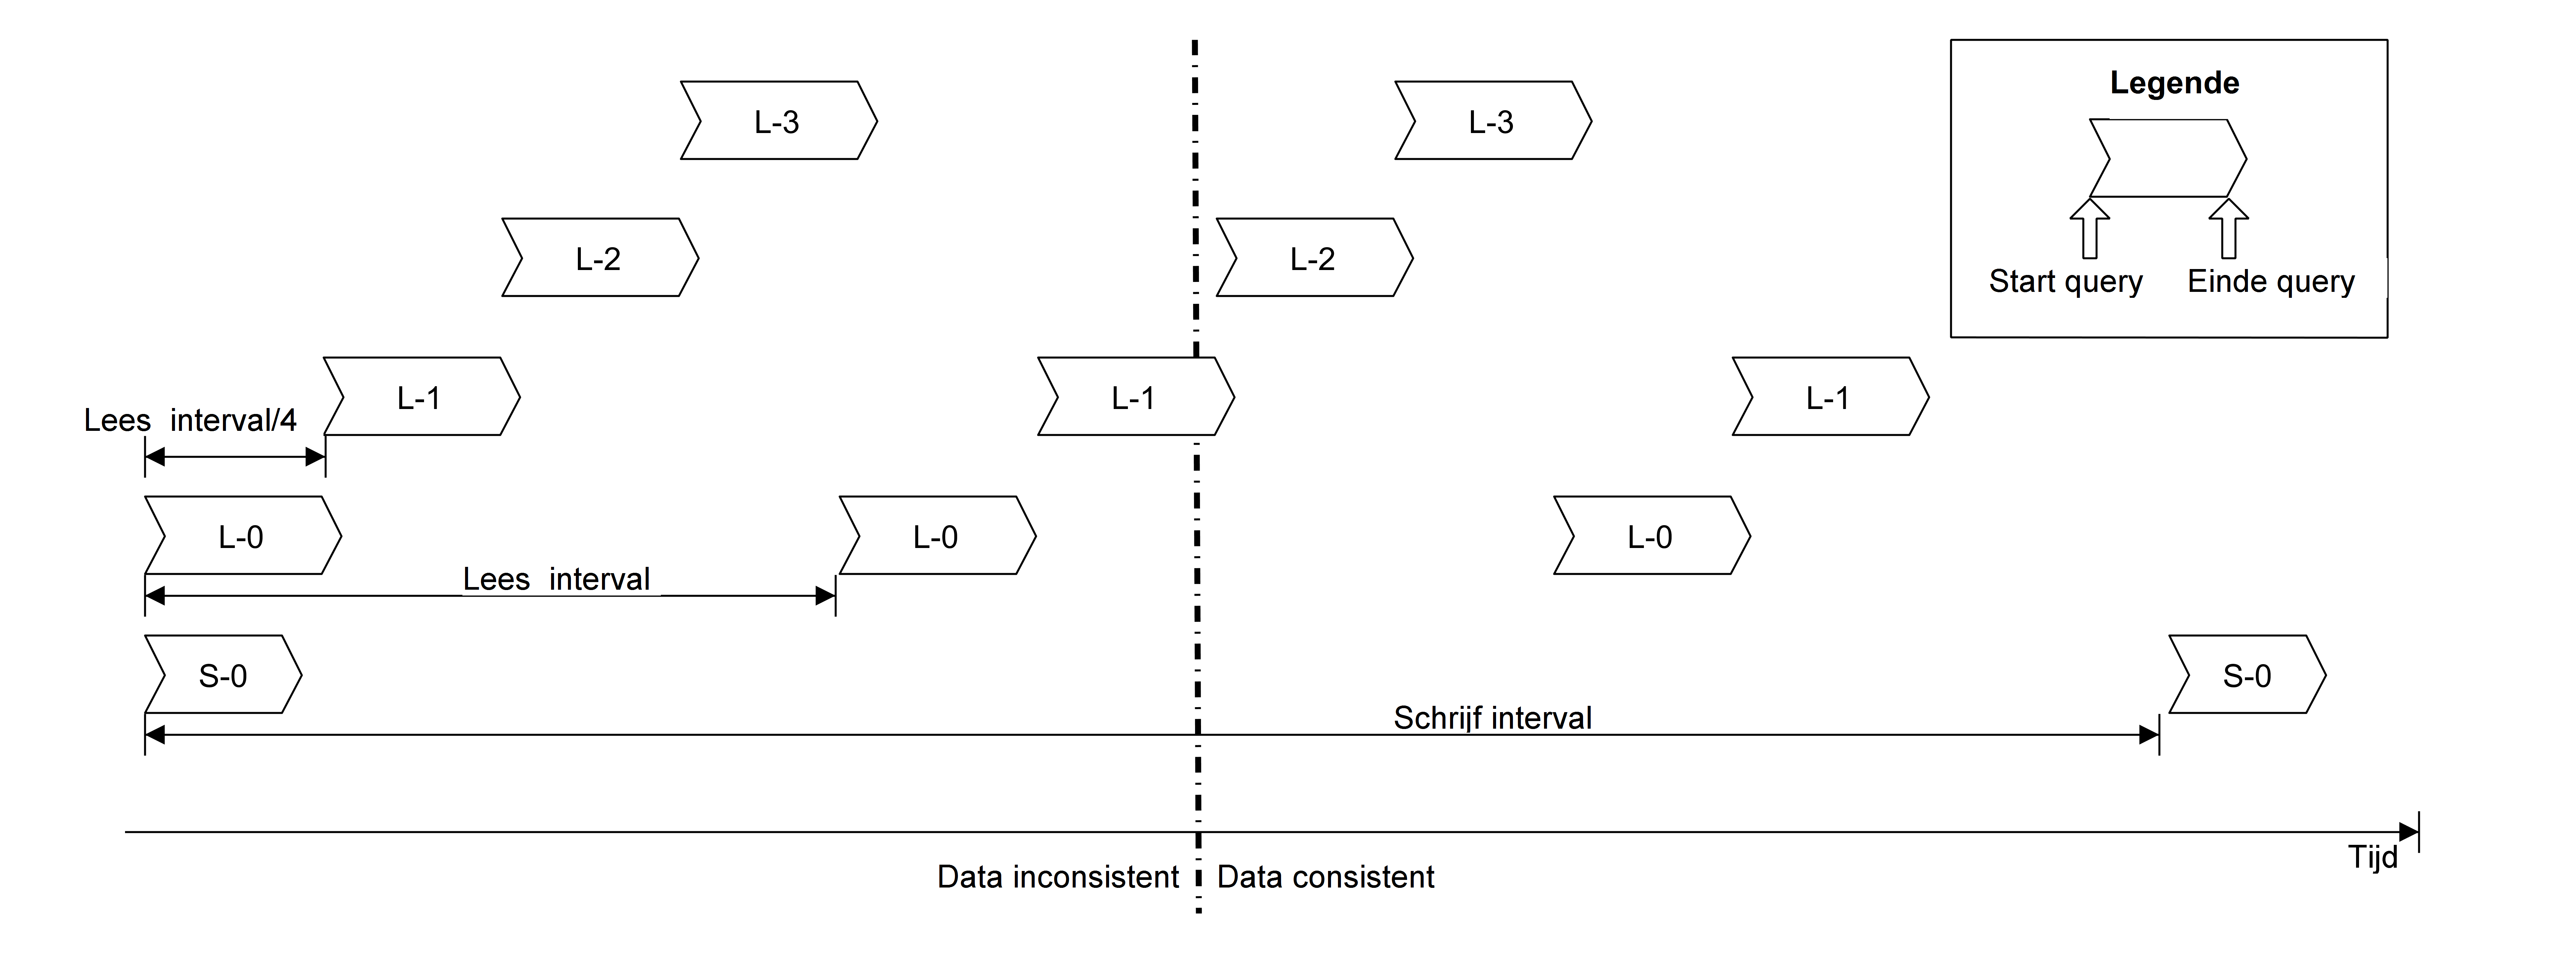
\includegraphics[width=\linewidth]{img/Consistentie-test-periode}
\caption{Consistentietest: Een enkele periode van de consistentietesten. Er is 1 schrijver, 4 lezers. De lezers stoppen zodra deze de data correct hebben gelezen. De rode lijn geeft aan vanaf wanneer de data consistent is voor alle queries gestart na dit tijdstip. }
\label{fig:test-consistentietest-periode}
\end{figure}


\subparagraph{Schatten van de basisbelasting} De basisbelasting kan de berekende belasting zijn in stap 2, waardoor het reëel aantal queries hoger ligt door de queries van de lezers en schrijver. De belasting kan ook verminderd worden met een geschat aantal queries die de schrijvers en lezers zullen uitvoeren. Het aantal queries van de schrijver en lezers per seconde kan berekend worden aan de hand van de hand van volgende formule: $(S + \#L*\#queriesperschrijfperiode / schrijfinterval$. Het aantal leesbewerkingen per schrijf periode zal geschat moeten worden, maar kan bijvoorbeeld op 1 gezet worden. Op deze manier krijgen systemen die geen onmiddellijke consistentie afdwingen een hogere belasting om de correcte waarde te lezen. Er zal dan twee of meer keren geprobeerd moeten worden. 

\paragraph{Soorten uiteindelijke consistentie} Met deze uitgevoerde testen en data kan aangetoond worden dat bepaalde systemen bepaalde uiteindelijke consistentie vereisten niet volgen. Het is mogelijk om met deze testen een tegenvoorbeeld te vinden dat aantoont dat een systeem een eigenschap niet garandeert. Maar het vinden van geen tegenvoorbeeld is geen bewijs van de eigenschap, maar kan wel een indicatie geven van de zeldzaamheid van de situatie. 

\subparagraph{Consistentie} Een systeem is niet consistent indien één van de lezers het nieuwe record of de update niet leest \textit{indien de leesactie gestart is na het voltooien van de schrijfactie}. Als dit voorkomt, gedraagt het systeem zich niet alsof er maar een enkele data-instantie is. 

\subparagraph{Read your own writes consistentie} Deze garantie kan ontkracht worden indien een schrijver na het voltooien van zijn schrijfbewerking zijn eigen data opvraagt en niet de nieuwste waarde leest. Dit kan dezelfde connectie gebruik voor de schrijfbewerking zijn of een andere bewerking, een gebruiker moet dus meerdere connecties kunnen aanmaken.  

\subparagraph{Session consistentie} Session consistentie is een verzwakking van de vorig eis. Het is nu slechts nodig om de data te lezen van een schrijfactie in een zelfde sessie, niet voor nieuwe sessies van dezelfde gebruiker. Dit kan ontkracht worden door met dezelfde connectie als de schrijver te lezen en de oude data te lezen. 

\subparagraph{Casual consistentie} Deze test kan uitgevoerd worden door de schrijver verschillende schrijfacties na elkaar te laten uitvoeren. De lezer leest de records in een bepaalde volgorde. Indien de gebruiker de data van een latere schrijfactie leest maar nog niet van een schrijfbewerking die vroeger voltooid was, is deze eigenschap niet gegarandeerd. De eis kan strenger gemaakt worden door de schrijver tussendoor niet te laten lezen, dit zou andere resultaten kunnen hebben.

\subparagraph{Monotonic Read consistentie} In deze test lees de lezer continue hetzelfde record. Eenmaal deze een nieuwe versie heeft gelezen, mag deze nooit meer oudere data lezen. Indien dit wel het geval is, is ook deze eigenschap niet gegarandeerd. 

Zoals beschreven hierboven, biedt deze aanpak de mogelijkheid aan om naast een actieve ook een passieve analyse te doen op de data. In deze thesis zal er gefocust worden op de \textit{read your own writes} en \textit{monotonic read} consistentie. 

\section{Stap 4: Verzamelen en analyseren van de testdata}
Na het uitvoeren van de testen, dient de informatie die verschillende schrijver en lezers hebben vergaard, samen gebracht te worden. Met de verwerking van deze informatie wordt bepaald hoe lang het duurt voor de data overal consistent is of om  tegenvoorbeeld te zijn voor een bepaalde consistentie categorie. Bij de beschikbaarheidstesten wordt er onderzocht hoe lang bepaalde bewerkingen onmogelijk zijn. Daarnaast wordt de gemiddelde vertraging tussen de normale situatie en de situatie met een service minder vergeleken voor de verschillende bewerkingen.  

Voor de testen worden verschillende grafieken gegenereerd van de aanwezige data, dit met de voor de hand liggende reden dat een figuur meer duidelijkheid brengt dan een tabel van cijfers. .  

\section{Conclusie}
In dit hoofdstuk werden de verschillende stappen van de testmethode besproken. In het totaal bestaat de test uit 4 verschillende stappen. 
Deze testmethode biedt de mogelijkheid om op een analytische manier verschillende systemen gelijkaardig te testen naar hun gedrag in consistentie en beschikbaarheid. In het volgende hoofdstuk zal de implementatie besproken worden. 
